\documentclass[tikz,border=3pt]{standalone}
\usepackage[utf8]{inputenc}
\usepackage[T1]{fontenc}
\usepackage{lmodern}
\renewcommand{\familydefault}{\sfdefault}
\usepackage{sansmath}\sansmath
\usepackage{chemfig}
\usepackage{pgfplots}\pgfplotsset{compat=1.18,/pgf/number format/use comma,/pgf/number format/1000 sep={.}}
\usetikzlibrary{arrows.meta,calc,positioning,decorations.pathmorphing,patterns}
% paleta del sitio
\definecolor{nar}{HTML}{E8680C}\definecolor{narc}{HTML}{FFB35C}\definecolor{hielo}{HTML}{FFF3E8}
\definecolor{tinta}{HTML}{1D1D1F}\definecolor{gris}{HTML}{6E6E73}\definecolor{lila}{HTML}{7C5CF0}
\definecolor{azul}{HTML}{2F6FD6}\definecolor{menta}{HTML}{17A673}\definecolor{coral}{HTML}{E8342A}
\tikzset{cel/.style={draw=gris,fill=hielo,line width=0.9pt},nuc/.style={draw=gris!70,line width=0.6pt},
fib/.style={gris!55,line width=0.35pt},eti/.style={font=\footnotesize,text=tinta,align=center},
num/.style={circle,draw=nar,fill=white,text=nar,font=\small\bfseries,inner sep=1.2pt,minimum size=13pt},
fl/.style={-{Stealth[length=2.6mm]},gris,line width=0.9pt}}
\begin{document}
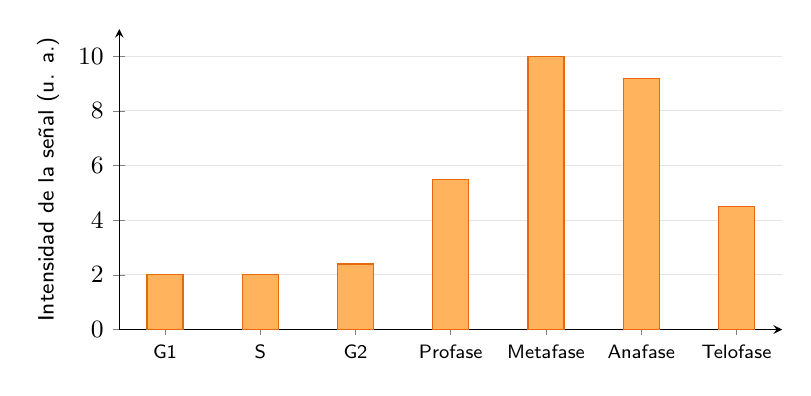
\begin{tikzpicture}[font=\small]
\begin{axis}[width=10cm,height=5.4cm,ybar,bar width=13pt,ymin=0,ymax=11,axis lines=left,enlarge x limits=0.08,
symbolic x coords={G1,S,G2,Profase,Metafase,Anafase,Telofase},xtick=data,x tick label style={font=\scriptsize},ytick={0,2,4,6,8,10},
ylabel={Intensidad de la señal (u. a.)},ylabel style={font=\footnotesize},ymajorgrids,grid style={gray!20}]
\addplot[fill=narc,draw=nar] coordinates {(G1,2) (S,2) (G2,2.4) (Profase,5.5) (Metafase,10) (Anafase,9.2) (Telofase,4.5)};
\end{axis}
\end{tikzpicture}
\end{document}
